\documentclass[10pt,a4paper]{article}

\usepackage[utf8x]{inputenc}
\usepackage[norsk]{babel}
\usepackage[T1]{fontenc,url}
\usepackage[hang,small,bf]{caption}
\usepackage{relsize}
\usepackage{setspace}
\usepackage{parskip}
\usepackage{lmodern}
\usepackage{microtype}
\usepackage{verbatim}
\usepackage{amsmath, amssymb, amsthm}
\usepackage{mathtools}
\usepackage{tikz}
\usepackage{physics}
\usepackage{algorithm}
\usepackage{algpseudocode}
\usepackage{listings}
\usepackage{enumerate}
\usepackage{graphicx}
\usepackage{float}
\usepackage{hyperref}
\usepackage{varioref}
\usepackage{todonotes}
\usepackage{color}
\usepackage{siunitx}
\usepackage[margin=1.5cm]{geometry}
\labelformat{equation}{ligning~(#1)}

\renewcommand{\exp}{\mathrm{e}^}
\newcommand{\halflife}{t_{\frac{1}{2}}}

\definecolor{light_green}{rgb}{0, 0.6, 0}
\definecolor{light_grey}{rgb}{0.5, 0.5, 0.5}
\definecolor{magenta}{rgb}{0.7, 0, 0.5}


\lstdefinestyle{py}{
    language = python,
    frame = single,
    showstringspaces = false,
    basicstyle = \small\ttfamily,
    breaklines = true,
    commentstyle = \color{light_grey},
    keywordstyle = \color{magenta},
    stringstyle = \color{light_green},
}


\begin{document}

\section*{Oppgave E.1}
Utfordringen ligger nok i hvordan de skal sette opp systemet dersom temperaturen til vannkokeren endrer seg. Ellers, er det viktig at de får med \texttt{legend} for å kunne skille mellom når vannet er i den ødelagte vannkokeren eller ei. 
\lstinputlisting[style=py]{boiling_water.py}
(Plot er på neste side) \hfill \\
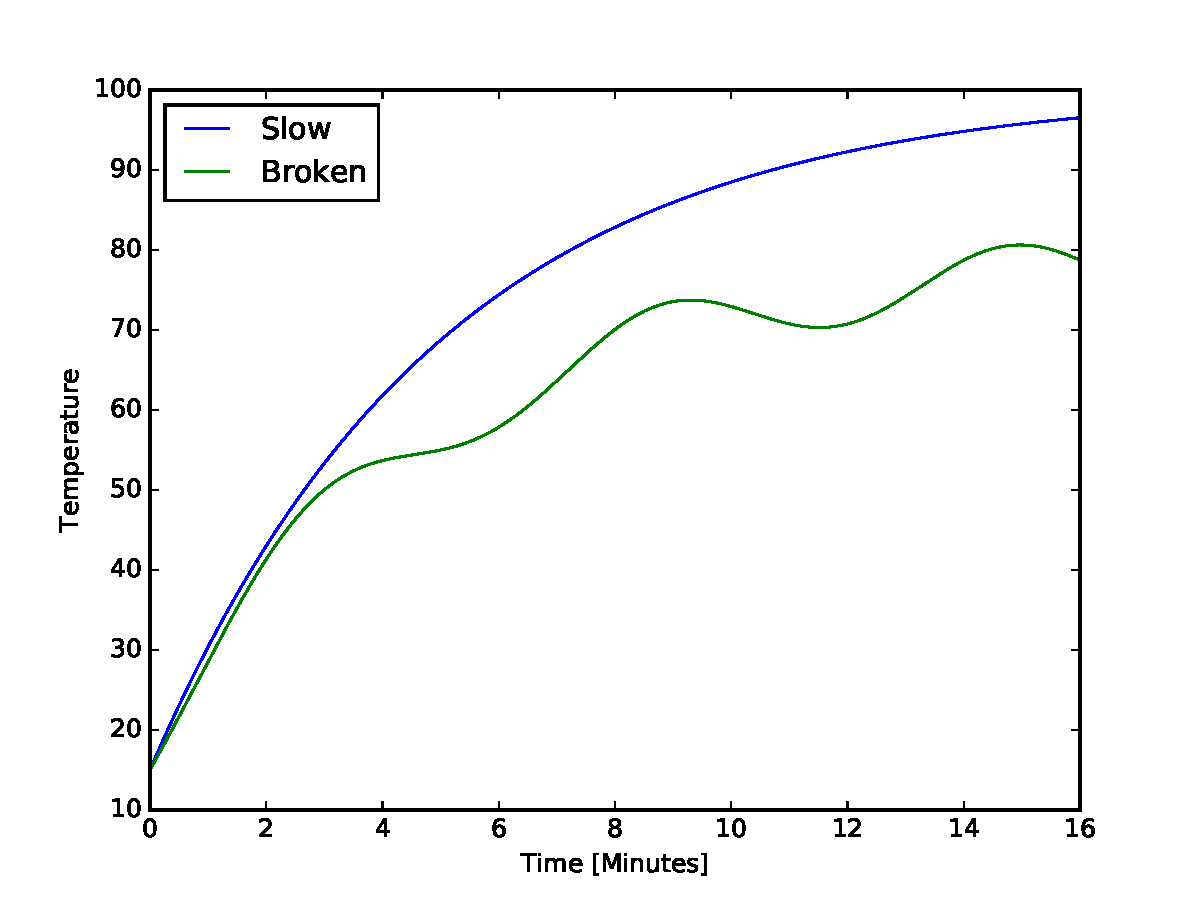
\includegraphics[scale=.75]{fig_boiling_water.pdf}

\newpage
\section*{Oppgave E.2}
ODE'en i a) er ganske straight forward. Bare å definere en funksjon for $Q(t)$, sette initialverdi, og løse.

I b) må Q omdefineres til å inneholde en if-test, som bestemmer $V$ for forskjellige tidspunkt. Utover det gjøres alt på indentisk måte.
\lstinputlisting[style=py]{RC.py}


\newpage
\section*{Oppgave E.3}
Her er det litt å passe på. Siden vi jobber nå i to dimensjoner (bevegelse langs x- og y-aksen), så må det passes på at det gjøres riktig oppsett av ODE-ene. Sidene som oppgaven referer til i boken, er veldig nyttige og hinter veldig mye til hvordan oppsettet skal være. 
\lstinputlisting[style=py]{throw_air_resistance.py}


\newpage
\section*{Oppgave E.4}
En vanlig feil vil sannsynligvis være å konvertere noen av enhetene tilbake til sekunder/meter/kg, som da gir gale resultater, med mindre man bytter alt tilbake til SI enheter. Dette vil gi rimelig gale resultater, men viser vel mest mangel på forståelse for fysikk, og ikke programmering.

Å implementere 2. ordens ODEs kan være en del mindre intuitivt å sette opp en 1. ordens, men det er egentlig bare å følge oppskriften gitt i boka. 
\lstinputlisting[style=py]{orbits.py}


\end{document}
